%\section{Project Management}
\chapter{Capabilities}
In this chapter we discuss the functionalities of Palladian in detail. The purpose of each section is to give a general understanding of how the algorithms work and how to use them practically.

\section{Classification}

\subsection{Text Classification}
Text classification is the process of assigning one or more categories to a given text document. There are several types of text classification which are shown in Figure \ref{fig:typesOfClassification}. Palladian can classify text in a single category, multiple categories, or in a hierarchical manner.

\begin{figure}[ht!]
\centering
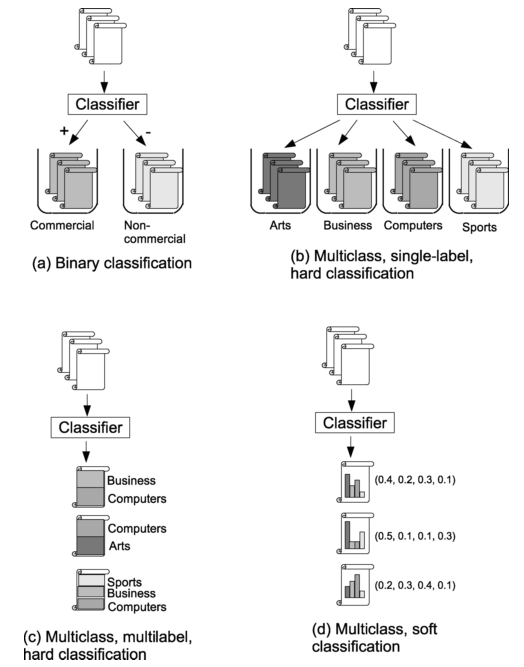
\includegraphics[width=4in]{img/typesOfClassification.png}
\caption{Types of classification\cite{qi2009web}.}
\label{fig:typesOfClassification}
\end{figure}

The text classification components are built from scratch and do not rely on external libraries such as Weka. In this section we will explain which features can be used for the classification, the basic theory of the classifiers, and how the performance of a classifier can be evaluated. In each section, we will describe theory and how the classification components can be used programmatically.

\subsubsection{Classification Type}
Palladian supports simple single category classification, tagging, and hierarchical classification. Each classifier needs to know in which type it has to perform classification.
This information is stored in the ClassificationTypeSetting object which is then passed to the classifier. Please read the Javadoc of that class for more detailed information.

\subsubsection{Features}
Features are the input for a classifier. In text classification we have a long string as an input from which we can derive several features. All of Palladian's classifiers work with n-grams. N-grams are sets of tokens of the length n. Palladian can preprocess text with character or word-level n-grams. See Section \ref{sec:ngrams} for more details.

Sometimes you do not want to have all n-grams to be features for the classifier. You can simply disallow certain features by putting them in a stop word list. These n-grams will then be ignored for the classification.

%CODE
All these settings are stored in a FeatureSetting object which is passed to the classifier. Please read the Javadoc of that class for more detailed information.

\subsubsection{Text Classifiers}
The text classifiers perform the actual classification task by calculating the most relevant category (or categories) for the input document. Two text classifiers are implemented, a dictionary based classifier and a k-nearest neighbor classifier. Both are explained in more detail in the following paragraphs.

\paragraph{K-Nearest Neighbor Text Classifier}
The KNN classifier uses the n-grams of the training documents to place them in a high dimensional vector space. The dimensions of the space equal the total number of available n-grams. Each training document is therefore a vector in that highly dimensional space. A new, unclassified document is now put into that vector space and by using distance function the k nearest neighbors are found for that document. Each of these neighbors votes with its own class, the more votes for one class the more likely that the new document belongs to that class.

\begin{figure}[ht!]
\centering
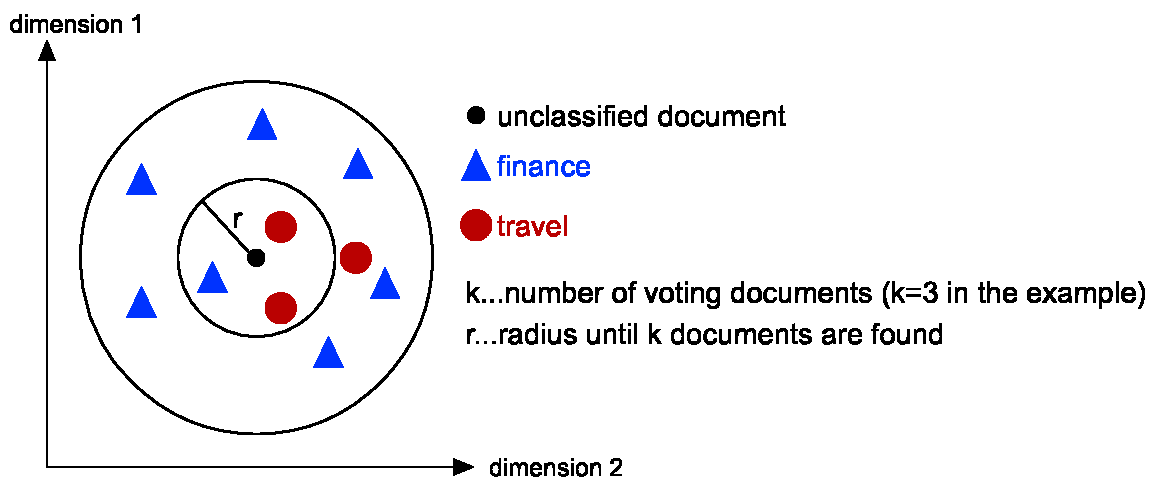
\includegraphics[width=0.8\textwidth]{img/knn.pdf}
\caption{A simple KNN example.}
\label{fig:knn}
\end{figure}

Figure \ref{fig:knn} shows a simple example of how the KNN classifier works. We limited the dimension to two for easier understanding. In this scenario we want to classify the given document (black dot in the middle) into one of the two categories ``finance'' (blue triangles) or ``travel'' (red dots). We calculate the distance between the new document and all training documents and consider the votes of the nearest three. In the example, two of these three document vote for ``travel'' which would let us classify our input document into that class.

The distance between two documents is calculated as shown in Equation \ref{eqn:knnDistance} where $d1$ and $d2$ are the two documents. The shorter the distance, the more similar the documents.

\begin{equation}
\label{eqn:knnDistance}
distance(d1,d2) = \frac{1}{numberOfMatchingNGrams}
\end{equation}

\paragraph{Dictionary-Based Classifier}
The dictionary-based classifier\footnote{This classifier won the first Research Garden (\url{http://www.research-garden.de}) competition where the goal was to classify product descriptions into 8 different categories. See press release at \url{http://www.research-garden.de/c/document_library/get_file?uuid=e60fa8da-4f76-4e64-a692-f74d5ffcf475&groupId=10137}} learns how probable each n-gram is for each given category and assigns the most probable category (or categories) to the input document.

A dictionary is built at training stage by counting and normalizing the co-occurrences of one n-gram and a category. The dictionary might then look as shown in Table \ref{tab:dictionary} where each column is a category (finance, travel, and science) and each row is an n-gram. In each cell we now have the learned relevance for each n-gram and category $relevance(ngram,category)$. The sum of the relevances in each row must add up to one.

Table \ref{tab:dictionary} shows an example dictionary matrix. The n-gram ``money'' is more likely to get the category ``finance'' ($relevance(money,finance) = 0.6$) than ``science'' ($relevance(money,science) = 0.25$) while the n-gram ``beach'' is most likely to appear in the category ``travel'' ($relevance(beach,travel) = 0.85$.

\begin{table}[ht]
\centering
\begin{tabular}{|l|l|l|l|}
\hline
n-gram   & finance & travel & science \\
\hline
money	   & 0.6	&	0.15	&	0.25	\\
\hline
beach	& 0.1	&	0.85	&	0.05	\\
\hline
paper	   & 0.3 &	0.2	&	0.5	\\
\hline
\end{tabular} 
\caption{N-Gram dictionary with relevances for categories.}
\label{tab:dictionary}
\end{table}

To classify a new document, we again create all n-grams, look up the relevance scores in the dictionary and assign the categories with the highest probability. The probability for each category and given document is calculated as shown in Equation \ref{eqn:dictionaryCategoryProbabilty} where $N_{Document}$ is the set of n-grams for the given document.

\begin{equation}
\label{eqn:dictionaryCategoryProbabilty}
\mbox{$CategoryProbability(category,document)$} = \sum_{n\,\epsilon\, Nurl} \mbox{$relevance(n,category)$}
\end{equation}

The dictionary can be stored in memory, in an embedded H2 database, or in a client/server MySQL database. These settings can be made in the classification.conf file in the conf folder (see Section \ref{sec:config.conf}).

%TODO category boost
%TODO cooccurrence

\subsubsection{Evaluation}
In order to find out which classifier works best with which feature settings, you can evaluate these combinations. The ws.palladian.classification.page.ClassifierManager has the $learnBestClassifier$ method to run the evaluation on all given classifiers with the given evaluation setting object ws.palladian.classification.page.EvaluationSetting. See Section \ref{sec:bpTextClassification} for more details of how to perform the evaluation programmatically.

The output of the evaluation will be three csv files that hold information about the combinations of classifier, dataset, training percentage, and the final performance for the combination. The performance is measured in precision, recall, and F1. The three files are stored in the data/temp folder and hold the following information.

\paragraph{averagePerformancesDatasetTrainingFolds.csv} This file holds the performance measures for each classifier, averaged over all given datasets, training percentages, and folds in the cross validation.

\paragraph{averagePerformancesTrainingFolds.csv} This file holds the performance measures for each classifier and dataset combination, averaged over all given training percentages and folds in the cross validation.

\paragraph{averagePerformancesFolds.csv} This file holds the performance measures for each classifier, dataset, and training percentage combination, averaged over all given folds in the cross validation.

\subsubsection{Best Practices}
\label{sec:bpTextClassification}
This section describes how to prepare training and testing data to learn a model, evaluate, and use a text classifier.

\paragraph{Preparing the Training/Testing Data}
The data can be specified in a simple text file. There are three classification options, namely, one-category classification, hierarchical classification and multi-category classification. They all require a similar structure of the data.

\subparagraph{One-Category Classification}
We write one URL and one category separated with a single space on each line. For example:
\begin{verbatim}
http://www.google.com search
http://www.fifa.com sport
http://www.oscars.com entertainment
\end{verbatim}

\subparagraph{Hierarchical Classification}
We write one URL and multiple categories separated with a single space on each line. The categories must be in the correct order, so the first category is the main one, all following are subcategories of each other. For example:
\begin{verbatim}
http://www.google.com search search_engine
http://www.fifa.com sport team_sports soccer 
http://www.oscars.com entertainment movies awards usa
\end{verbatim}

\subparagraph{Multi-Category Classification}
We write one URL and multiple categories separated with a single space on each line. The order of the categories (tags) does not matter. For example:
\begin{verbatim}
http://www.google.com search image_search video_search
http://www.fifa.com soccer sport free_time fun ball_game results to_read
http://www.oscars.com entertainment movies films awards watch video stars
\end{verbatim}

\paragraph{Training a classifier}
Before we can use a classifier, we need to learn a model. The model is an internal representation of the learned data. After learning a model, a classifier can applied to unseen data. We now have prepared the training and testing data so we can now learn the models.
The classifier is saved as a lucene index or a database under the name of the classifier with a ``Dictionary'' suffix. The result of the learning are three files: the classifier (``CLASSIFIER.ser''), the dictionary object (``CLASSIFIERDictionary.ser''), and the actual dictionary as the index or database (e.g. ``CLASSIFIERDictionary.h2.db''). More settings can be configured in the config/classification.conf file. See \ref{sec:classification.conf} for more information.

Listing \ref{listing:trainClassifier} shows an example for how to train and save a classifier. In this case we train a classifier that can classify the language of given documents. As training data we use a list of web pages of different languages from Wikipedia.

\begin{codelisting}
\begin{lstlisting}[label=listing:trainClassifier,caption=Training a classifier.,frame=tb]
// create a classifier mananger object
ClassifierManager classifierManager = new ClassifierManager();

// specify the dataset that should be used as training data
Dataset dataset = new Dataset();

// set the path to the dataset
String dsPath = "data/datasets/classification/language/index.txt";
dataset.setPath(dsPath);

// tell the preprocessor that the first field in the file is a link to 
// the actual document
dataset.setFirstFieldLink(true);

// create a text classifier by giving a name and a path 
// where it should be saved to
String dcn = "LanguageClassifier";
String dcp = "data/models/languageClassifier/";
TextClassifier classifier = new DictionaryClassifier(dcn,dcp);

// specify the settings for the classification
ClassificationTypeSetting cts = new ClassificationTypeSetting();

// we use only a single category per document
cts.setClassificationType(ClassificationTypeSetting.SINGLE);

// we want the classifier to be serialized in the end
cts.setSerializeClassifier(true);

// specify feature settings that should be used by the classifier
FeatureSetting featureSetting = new FeatureSetting();

// we want to create character-level n-grams
featureSetting.setTextFeatureType(FeatureSetting.CHAR_NGRAMS);

// the minimum length of our n-grams should be 3
featureSetting.setMinNGramLength(3);

// the maximum length of our n-grams should be 5
featureSetting.setMaxNGramLength(5);

// we assign the settings to our classifier
classifier.setClassificationTypeSetting(classificationTypeSetting);
classifier.setFeatureSetting(featureSetting);

// now we can train the classifier using the given dataset
classifierManager.trainClassifier(dataset, classifier);
\end{lstlisting}
\end{codelisting}

\paragraph{Using a classifier}
After we trained a model for a classifier we can apply it to unseen data. Let's use the model we just trained to classify the language of a new document.

Listing \ref{listing:useClassifier} shows how to use a trained classifier.

\begin{codelisting}
\begin{lstlisting}[label=listing:useClassifier,caption=Use a trained text classifier.,frame=tb]
// the path to the classifier we want to use
String path = "data/models/languageClassifier/LanguageClassifier.ser";

// load the language classifier
TextClassifier classifier = ClassifierManager.load(path);

// create a classification document that holds the result
ClassificationDocument classifiedDocument = null;

// classify the little text (if classifier works it would say Spanish)
classifiedDocument = classifier.classify("Yo solo s� que no s� nada.");

// print the classified document
System.out.println(classifiedDocument);
\end{lstlisting}
\end{codelisting}

You can also try the language classifier online at \url{http://www.webknox.com/wi#detectLanguage}.

\paragraph{Evaluating a Classifier}
To get an idea of how good a trained classifier works, we can evaluate it using test data which is structured the same way as the training data. Listing~\ref{listing:evaluateClassifier} shows how to evaluate a trained classifier, you will see that is very similar to training a classifier. Make sure that you evaluate the classifier using disjunct data, otherwise the evaluation results are invalid .

\begin{codelisting}
\begin{lstlisting}[label=listing:evaluateClassifier,caption=Evaluating a trained text classifier.,frame=tb]
// create a classifier mananger object
ClassifierManager classifierManager = new ClassifierManager();

// the path to the classifier we want to use
String path = "data/models/languageClassifier/LanguageClassifier.ser";

// specify the dataset that should be used as testing data
Dataset dataset = new Dataset();

// the path to the dataset (should NOT overlap with the training set)
dataset.setPath("data/datasets/classification/language/index.txt");

// tell the preprocessor that the first field in the file is a link
// to the actual document
dataset.setFirstFieldLink(true);

// load the language classifier
TextClassifier classifier = ClassifierManager.load(path);

// now we can test the classifier using the given dataset
ClassifierPerformance classifierPerformance = null;
classifierManager.testClassifier(dataset, classifier);
\end{lstlisting}
\end{codelisting}

\paragraph{Testing parameter combinations}
As you have seen, you can train the classifier using different parameters. So how can you be sure that you set the parameters correctly? Do they work well on different datasets? Is the chosen classifier always better than others? In order to answer these questions with hard data you can automatically run different combinations of classifiers, settings, and datasets as shown in Figure \ref{fig:bcc}. The green line shows the combination that was found to perform best. In the end you will get one evaluation csv with information about how the combination performed. You can then manually pick the best performing settings.

\begin{figure}[ht!]
\centering
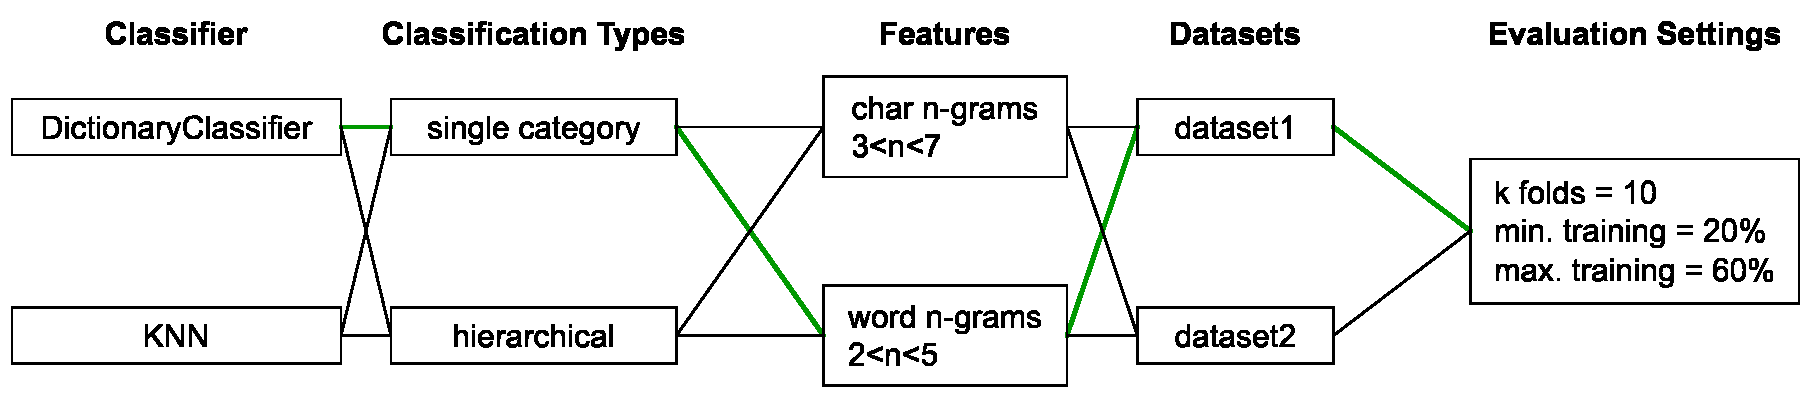
\includegraphics[width=\columnwidth]{img/bcc.pdf}
\caption{Combinations for training a solid classifier.}
\label{fig:bcc}
\end{figure}

Listing \ref{listing:bcc} shows you how to do just that.

\begin{codelisting}
\begin{lstlisting}[label=listing:bcc,caption=Learning the best parameter combination for a text classifier.,frame=tb]
ClassifierManager classifierManager = new ClassifierManager();

// build a set of classification type settings to evaluate
List<ClassificationTypeSetting> ctsList;
ctsList = new ArrayList<ClassificationTypeSetting>();
ClassificationTypeSetting cts = new ClassificationTypeSetting();
cts.setClassificationType(ClassificationTypeSetting.SINGLE);
cts.setSerializeClassifier(false);
ctsList.add(cts);

// build a set of classifiers to evaluate
List<TextClassifier> classifiers = new ArrayList<TextClassifier>();
TextClassifier classifier = null;
classifier = new DictionaryClassifier();
classifiers.add(classifier);
classifier = new KNNClassifier();
classifiers.add(classifier);

// build a set of feature settings for evaluation
List<FeatureSetting> featureSettings = new ArrayList<FeatureSetting>();
FeatureSetting fs = null;
fs = new FeatureSetting();
fs.setTextFeatureType(FeatureSetting.CHAR_NGRAMS);
fs.setMinNGramLength(3);
fs.setMaxNGramLength(7);
featureSettings.add(fs);

fs = new FeatureSetting();
fs.setTextFeatureType(FeatureSetting.CHAR_NGRAMS);
fs.setMinNGramLength(2);
fs.setMaxNGramLength(5);
featureSettings.add(fs);

fs = new FeatureSetting();
fs.setTextFeatureType(FeatureSetting.WORD_NGRAMS);
fs.setMinNGramLength(2);
fs.setMaxNGramLength(5);
featureSettings.add(fs);

// build a set of datasets that should be used for evaluation
Set<Dataset> datasets = new HashSet<Dataset>();
Dataset dataset = new Dataset();
dataset.setPath("dataset1.txt");
datasets.add(dataset);
dataset = new Dataset();
dataset.setPath("dataset2.txt");
dataset.setSeparationString("#");
datasets.add(dataset);

// set evaluation settings
EvaluationSetting evaluationSetting = new EvaluationSetting();
evaluationSetting.setTrainingPercentageMin(20);
evaluationSetting.setTrainingPercentageMax(80);
evaluationSetting.setkFolds(5);
evaluationSetting.addDataset(dataset);

// let's take the time
StopWatch stopWatch = new StopWatch();

// train and test all classifiers in all combinations
classifierManager.learnBestClassifier(ctsList, classifiers, 
                                      featureSettings,
                                      evaluationSetting);

System.out.println("finished training and testing classifier
          combinations in " + stopWatch.getElapsedTimeString());
\end{lstlisting}
\end{codelisting}

\subsection{Language Detection}
Language detection is the task of determining the language of a given text. In the last section we explained how a text classifier can be trained. We used this training method to learn a dictionary based classifier for language detection and evaluated it against other state-of-the-art algorithms.
We compared our algorithm to JLangDetect \cite{jlangdetect}, Google Translation API \cite{googleTranslationAPI}, and the Alchemy API \cite{alchemyLanguageAPI}. We used the Multilingual Parallel Corpus of the Joint Research Centre of the European Commission in version 3.0 \cite{jrcCorpus}. This corpus contains about half a million documents in 22 languages about politics. Since we could not train the language detectors from Google and Alchemy, the comparison is not fair to both of them but we put the results here to see how they are performing with their classifiers. Due to API restrictions we had to crop the length of the text to maximum of 100 characters.
We trained both, JLangDetect and Palladian on a sample of 100 documents per language. JLangDetect was trained with character level n-grams between one and three\footnote{This setting has been said to be work well by the author of the JLangDetect, see \url{http://www.jroller.com/melix/entry/nlp_in_java_a_language}} while Palladian was trained with word level n-grams between one and three. We then tested all algorithms an a test set containing again 100 documents per language. Since the classifier performance is very sensitive to the length of the given text, we evaluated all algorithms with short texts ($\leq$ 10 characters), medium texts ($\leq$ 30 characters), and long texts (no length limitation, but usually about 20 to 200 sentences).
Table \ref{tab:languageDetectionEvaluation} shows the evaluation results. All results in brackets are not representative since many documents were not classified by the API.

\begin{table}[ht]
\centering
\begin{tabular}{|l|c|c|c|}
	\hline
	System & Short Texts & Medium Texts & Long Texts \\ 
	\hline
	JLangDetect & \textbf{74.64\%} & 87.91\% & 99.64\% \\ 
	\hline
	Alchemy API & (97.78\%) & 69.35\% & (88.27\%) \\ 
	\hline
	Google API & 57.32\% & 80.44\% & (99.21\%) \\ 
	\hline
	Palladian & 62.36\% & \textbf{88.18\%} & \textbf{99.91\%}  \\ 
	\hline
\end{tabular}
\caption{Evaluation results for language detection systems.}
\label{tab:languageDetectionEvaluation}
\end{table}

As we can see, JLangDetect performs very well across all text lengths. Palladian is, however, slightly superior as soon as the text length is longer than about 10 to 20 characters.

\section{Extraction}

%TODO refactor from "ControlledTagger" to "ControlledKeywordExtractor" or something like that..
\subsection{Keyword Extraction / Controlled Tagging}
It is often interesting which words describe a given text most. These words are often called ``keywords'' or ``tags''. Palladian is able to use a weighted, controlled vocabulary and perform tagging of a text using TF-IDF and tag correlations.

The ControlledTaggerIndex is the basis for the tagging. This index contains information about the controlled tag vocabulary, tag frequencies, a stem-map, and a correlation table for all tags. The tag index is built using training data of single text files that have been assigned with weighted tags. This index can be serialized as a model file for later usage.

To tag a new text with the most relevant keywords, the ControlledTagger tokenizes the input text and stems the tokens, which means that tokens like ``blogging'' and ``blogs'' are consolidated to the common term ``blog''.

All tokens that match a tag from the controlled vocabulary in the index are held in a bag-of-words which also stores the frequencies of the tokens in the input text. Using this data, we can calculate the TF-IDF values for each tag candidate. The TF-IDF scores are used to rank the tags initially. The determined tag candidates are then processed by two re-ranking steps to improve the final results:

\begin{description}

	\item [Prior probabilities] considers the probability of a tag occuring in the training data. This way, more popular tags are prioretized.

	\item [Correlations] considers the probability of a specific pair of tags co-occuring in the training data. For example, the trained model might suggest a strong correlation between the pair ``apple'' and ``iphone''. The strenghts of such correlations can be taken into account for the re-ranking.

\end{description}

% TODO insert figure from thesis about re-ranking here?

ControlledTagger was designed to be trained with large amounts of manually tagged documents. For our experiments we relied on the DeliciousT140 dataset which can be obtained from \cite{deliciousT140}. The dataset was crawled from Delicious and contains over 140.000 tagged documents. For convenient access to the dataset, Palladian provides the class DeliciousDatasetReader. The DeliciousDatasetReader gives access to the XML-based dataset and supports various filter operations. For a usage example please take a look at the main method of the class.

The ControlledTagger can be configured using the ControlledTaggerSettings class. You can configure the following aspects:

\begin{enumerate}
\item TF-IDF threshold under which the tags should be discarded or alternatively, the number of fixed tags per document.
\item The correlation re-ranking modus.
\item The stemmer to use. We can choose between different SnowballStemmer implementations for various natural languages. For further informations about Snowball, please consult \cite{snowball}.
\item The stop words list.
\item A list of regular expression that the tags need to match in order to be assigned.
\end{enumerate}

Listing~\ref{listing:trainControlledTagger} shows the training of the ControlledTagger with data from Delicious and the finally the serialization of the trained model.

\begin{codelisting}
\begin{lstlisting}[label=listing:trainControlledTagger,caption=Training the controlled tagger.,frame=tb]
// set up the ControlledTagger
final ControlledTagger tagger = new ControlledTagger();
        
// tagging parameters are encapsulated by ControlledTaggerSettings
ControlledTaggerSettings taggerSettings = tagger.getSettings();
        
// create a DeliciousDatasetReader + Filter for training
DeliciousDatasetReader reader = new DeliciousDatasetReader();
DatasetFilter filter = new DatasetFilter();
filter.addAllowedFiletype("html");
filter.setMinUsers(50);
filter.setMaxFileSize(600000);
reader.setFilter(filter);
        
// train the tagger with 20.000 train documents from the dataset
DatasetCallback callback = new DatasetCallback() {
    @Override
    public void callback(DatasetEntry entry) {
        String content = FileHelper.readFileToString(entry.getPath());
        content = HTMLHelper.htmlToString(content, true);
        tagger.train(content, entry.getTags());
    }
};
reader.read(callback, 20000);
        
// save the model for later usage
tagger.save("data/models/controlledTaggerModel.ser");
\end{lstlisting}
\end{codelisting}

Listing~\ref{listing:useControlledTagger} shows how to load a trained model into the ControlledTagger and use it for tagging text contents.

\begin{codelisting}
\begin{lstlisting}[label=listing:useControlledTagger,caption=Using the controlled tagger.,frame=tb]
ControlledTagger tagger = new ControlledTagger();

// load the trained model, this takes some time;
// if you will tag multiple documents, 
// make sure to move this outside the loop!
tagger.load("data/models/controlledTaggerModel.ser");
        
// assign tags according to a web page's content
PageContentExtractor extractor = new PageContentExtractor();
String content = extractor.getResultText(
	"http://arstechnica.com/open-source/news/2010/10/" + 
	"mozilla-releases-firefox-4-beta-for-maemo-and-android.ars");
List<Tag> assignedTags = tagger.tag(content);
        
// print the assigned tags
CollectionHelper.print(assignedTags);
\end{lstlisting}
\end{codelisting}

The keyword extraction is state-of-the-art and beats the comparable system ``Maui''\cite{medelyan2009human} by 18.9\% in the F1-Score.
More information about the controlled tagging can be found in \cite{katz2010diploma}.

\subsection{Web Page Content Extraction}
Content oriented web pages such as blogs or news articles contain not only the text of interest but also clutter such as the navigation, footer, header, and ads. In order to automatically process the text without the clutter, we need to extract the text content. Figure \ref{fig:webpagecontentextractor} shows an example web page where the main article is in the green box. Everything else is just clutter and should not be extracted when looking for the unique article.

\begin{figure}[ht!]
\centering
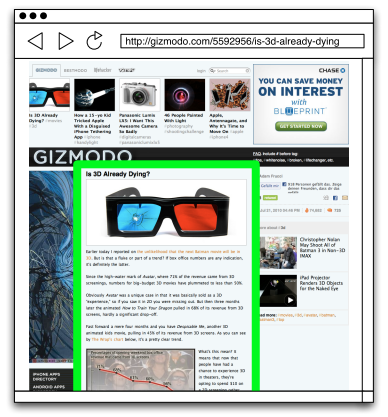
\includegraphics[width=4in]{img/webpagecontentextractor.png}
\caption{Article content of a web page marked with a green box  \cite{katz2010diploma}.}
\label{fig:webpagecontentextractor}
\end{figure}

To perform this kind of extraction we could use wrapper approaches which are explained in more detail in \cite{ckgs2006}. However, these approaches require manual wrapper construction or semi-supervised learning which is too cumbersome.
Another approach would be to detect the template of the web page and get only the contents of the main block (the green box). Template detection usually works by comparing one page with several other pages of the same domain to find the fix and changeable contents. A template based approach is available in Palladian, check chapter \ref{sec:WebPageTemplateDetection}. This however requires several HTTP requests and therefore more time and bandwidth.

Palladian offers two approaches together with thier corresponding implementations which are based on analyzing single pages and employing certain heuristics to identify relevant sections of web pages:

\begin{description}
	
	\item \texttt{PalladianContentExtractor} extracts clean sentences from (English) texts. While short phrases are not included in the output, this approach will extract all readable content from a page without distinguishing specific page areas, like content or comment sections.
	
	\item \texttt{ReadabilityContentExtractor} is more focused on general content. It works on the page's DOM trees; each DOM element is analyzed and ranked based on the length of the contained text, the link density, and the frequency of other elements in relation to the text length. Longer text fragments usually indicate a relevant part of the article, while a high link density is more likely to indicate that the analyzed element is part of the navigation for example. Also the attributes ``id'' and ``class'' are analyzed. If the attribute values contain keywords such as ``entry'', ``content'', or ``text'', the element is more likely to contain relevant content as if the attribute values contain keywords such as ``header'', ``footer'', or ``sidebar''. The implementation of the web page content extraction adopted great parts of the Firefox extension ``Readability''\footnote{\url{http://lab.arc90.com/experiments/readability/}}\footnote{By now, a bunch of alternative Java-based Readability ports are available:\\ \url{https://github.com/ifesdjeen/jReadability},\\ \url{https://github.com/basis-technology-corp/Java-readability},\\ \url{https://github.com/karussell/snacktory}}. The used heuristics in Readability have shown to be quite accurate for a wide range of web pages.
	
\end{description}

Additionaly, Palladian provides a wrapper class for Boilerpipe\footnote{\url{http://code.google.com/p/boilerpipe/}}, a Java library which is based on the algorithms described in \cite{BoilerplateDetectionShallowTextFeatures}. This gives Palladian's user the possibility to access three different content extraction techniques via a common interface. Listing~\ref{listing:usePageContentExtractor} gives a short usage example.

\begin{codelisting}
\begin{lstlisting}[label=listing:usePageContentExtractor,caption=Using the PageContentExtractor.,frame=tb]
WebPageContentExtractor extractor = new ReadabilityContentExtractor();
// or
// WebPageContentExtractor extractor = new PalladianContentExtractor();
// WebPageContentExtractor extractor = new BoilerpipeContentExtractor();

String url = "http://www.wired.com/gadgetlab/2010/05/iphone-4g-ads/";

// this method is heavily overloaded and accepts various types of input
extractor.setDocument(url);

// get the main content as text representation
String contentText = extractor.getResultText();

// get the main content as DOM representation
Document contentDocument = extractor.getResultDocument();

// get the title
String title = extractor.getResultTitle();
\end{lstlisting}
\end{codelisting}

We evaluated our Readability-inspired approach against Boilerpipe. For evaluation we used the ``L3S-GN1'' data set which is provided by the authors of Boilerpipe and consists of 621 manually annotated web pages with news articles from 408 different sites. The annotations which were assigned by humans categorize areas of web pages into different groups ``Headline'', ``Full text'',  ``Supplemental'', ``Related content'', ``Comments'' and  ``Not content'', where ``Full text'' represents the main article content of a web page (green box in figure~\ref{fig:webpagecontentextractor}).

We used both content extraction approaches on the data set and scored their results by comparing their extracted text content with the human extracted content using Levenshtein\footnote{\url{http://www.merriampark.com/ld.htm}} similarity. Table~\ref{tab:pageContentExtractionResults} shows the results of our evaluation. The number of wins denotes how many times one approach achieved a better e. g. more similar result than the other.


\begin{table}[ht]
\centering
\begin{tabular}{|l|c|c|c|}
	\hline
	System & Average Similarity & \# Wins & \# Errors \\ 
	\hline
	Boilerpipe (\texttt{ArticleExtractor}, version 1.1) & 88.93\% & 143 & 6 \\ 
	\hline
	Readability port (SVN revision 1444) & 90.91\% & 474 & 2 \\ 
	\hline
\end{tabular}
\caption{Evaluation results for web page content extraction approaches.}
\label{tab:pageContentExtractionResults}
\end{table}

\subsection{Web Page Template Detection}
\label{sec:WebPageTemplateDetection}

\subsection{Named Entity Recognition}

{\it Named Entity Recognition} (NER) is the task of recognizing and disambiguating known and unknown entities in documents. In order to understand the task we need to understand what an {\it entity} is. An entity is a collection of rigidly designated chunks of text that refer to exactly one or multiple identical, real or abstract concept instances. These instances can have several aliases and one name can refer to different instance \cite{webknoxblogne}. So for example ``Iron Man 2'' and ``Iron-Man 2'' are two different chunks of text which however refer to the same movie. Common types of entities are people (e.g. ``Jim Carrey''), locations (e.g. ``Los Angeles''), and organizations (e.g. ``Google Inc.'').

A named entity recognizer is therefore a system or technique that tries to detect entities in a given natural language text. For example, an NER system that is used to detect people, locations, and organizations should be able to find the bold entities in the following text:

\textbf{Bill Gates} founded \textbf{ Microsoft} with \textbf{ Paul Allen} in 1975 in \textbf{ Albuquerque, New Mexico}. The headquarter is located in \textbf{ Redmond, Washington} and the company is led by CEO \textbf{ Steve Ballmer}.

\subsubsection{Taggers}
Palladian wraps 8 Named Entity Recognizers using a single interface making it easier to test and substitute them in real world applications.

\paragraph{Alchemy} The Alchemy API is a web-based service that also offers Named Entity Recognition. Using this NER requires the application to have a developer key and Internet access. Alchemy covers a wide range of concepts. For more details see \url{http://www.alchemyapi.com/api/entity/types.html} or the JavaDoc.

\paragraph{Illinois Learning-based Java} Students from the University of Illinois developed this Recognizer \cite{illinoisccg}. The recognizer comes with a large set of lists that help the recognizer to tag concepts such as corporations, countries, jobs, movies, people, songs, and more. More information can also be found on \url{http://l2r.cs.uiuc.edu/~cogcomp/asoftware.php?skey=FLBJNE}.

\paragraph{Julie} The Julie Lab of the University of Jena added a named entity recognizer to their NLP toolsuite \cite{hahn2008overview}. The tagger is based on conditional random fields and comes with three models from the biomedical domain. Other models can however trained using Palladian. For more information see the pdf which is contained in their stand-alone download from \url{http://www.julielab.de/Resources/Software/NLP+Tools/Download/Stand_alone+Tools.html}.

\paragraph{LingPipe} The LingPipe library \cite{lingpipe} also offers an NER. Unfortunately the tagger comes with no models. Models for each desired concept need to be trained manually. More information can be found on \url{http://alias-i.com/lingpipe/demos/tutorial/ne/read-me.html}.

\paragraph{OpenCalais} The Open Calais API \cite{opencalais} is a web-based service that also offers Named Entity Recognition. The service requires a developer key and access to the Internet. Open Calais covers many concept as covered on the documentation \url{http://www.opencalais.com/documentation/calais-web-service-api/api-metadata/entity-index-and-definitions} and in the JavaDoc.

\paragraph{OpenNLP} The OpenNLP toolkit \cite{opennlp} provides a maximum entropy based approach for named entity recognition. The toolkit comes with a small set of pre-trained models covering concepts such as locations, organizations, and persons. More details can be found in the JavaDoc.

\paragraph{Stanford} As part of the Stanford NLP library \cite{stanfordnlp, finkel2005stanfordner} developed a named entity recognizer that is based on conditional random fields (CRF). The tagger was trained on the CoNLL 2003 data and comes with a small set of classifiers that can recognize persons, locations, and organizations. For more details see \url{http://www-nlp.stanford.edu/software/crf-faq.shtml} and the JavaDoc.

\paragraph{TUD} The TUD named entity recognizer was developed at the Dresden University of Technology. The recognizer is based on a list lookup and dictionary classification approach. So far no trained models exist for this tagger.

\subsubsection{Tagging a Text}
To use an NER you need two things: A text that you want to tag and a model for the tagger that has been trained to recognize the entities you want to find in the given text.
The tagging works the same for all NERs and is shown in Listing \ref{listing:useNER}.

\begin{codelisting}
\begin{lstlisting}[label=listing:useNER,caption=Tagging a text using a named entity recognizer.,frame=tb]
// create the tagger
NamedEntityRecognizer ner = new TUDNER();

// the text to be tagged
String inputText = "The iphone 4 is the successor of the iphone 3gs.";

// the path to the model which should be used for tagging
String modelPath = "data/models/tudner/phone.model";

// tag the text using the specified model
String taggedText = ner.tag(inputText, modelPath);
System.out.println(taggedText);
// desired output
// The <PHONE>iphone 4</PHONE> is the successor
// of the <PHONE>iphone 3gs</PHONE>.

// avoid loading the model each time using it
ner.loadModel("data/models/tudner/phone.model");
ner.tag(inputText);
\end{lstlisting}
\end{codelisting}

In order to find out which tags were trained for the model you can create a meta file with one tag name per line, give it the same name as the model adding the suffix ``\_meta'' and save it as a text file next to the model. Listing \ref{listing:nerMeta} shows how you can get a list of tags that a model can apply.

\begin{codelisting}
\begin{lstlisting}[label=listing:nerMeta,caption=Reading a model's meta data.,frame=tb]
// create the tagger
NamedEntityRecognizer ner = new TUDNER();

// the meta file must be called phone_meta.txt
List<String> tags = ner.getModelTags("data/models/tudner/phone.model");

// print the tags to the console
CollectionHelper.print(tags);
\end{lstlisting}
\end{codelisting}

\subsubsection{Training a Tagger}

Some of the available taggers come with trained models that can be used to detect entities. However, the concepts they were trained for might not be sufficient for the application you have in mind, therefore, you need to create your own training set with entities from your domain and learn a tagger using that data. This section explains which tagging formats are available and how models for the available taggers can be trained.

First we start with the tagging formats which can be used to create a training set.

\paragraph{Tagging Formats}
Many tagging types have been developed which makes interoperability between different systems harder. Palladian can handle many of these formats and is able to transform a tagged text within these formats. 

The different tagging are explained in this section using the same example text: ``Bill Gates founded Microsoft in 1975.''.

\subparagraph{Slash} The slash notation tags a given text with a slash and the tag right after the word. The sample text in the slash notation would look as show below.

\begin{verbatim}
Bill/PERSON Gates/PERSON founded Microsoft/ORG in 1975/DATE.
\end{verbatim}

\subparagraph{Bracket} The bracket notation wraps the word in brackets. The sample tags would look as shown below.

\begin{verbatim}
[Bill Gates PERSON] founded [Microsoft ORG] in [1975 DATE].
\end{verbatim}

\subparagraph{Column (BIO)} The column notation is one of the most widely used. For example the CoNLL NER dataset uses this format. The text is tokenized and on each line of the tagged text there is only one token (word) with its related tag separated by a space or tab. The BIO format means \textbf{ B}eginning, cont\textbf{ I}nue, and \textbf{ O}utside. The BIO format can help to distinguish entities of the same type that are written close together.

The sample text in the column format would look as shown below. The ``O'' tag stands for ``outside'', that is no matching tag has been found.

\begin{verbatim}
Bill PERSON
Gates PERSON
founded O
Microsoft ORG
in O
1975 DATE
. O
\end{verbatim}

The sample text in the column BIO format would look as shown below.

\begin{verbatim}
Bill B-PERSON
Gates I-PERSON
founded O
Microsoft B-ORG
in O
1975 B-DATE
. O
\end{verbatim}

If we had another person name right after the first one, our tagger might think that it was only one person if we use the column notation. In the column BIO notation, both persons could be distinguished because the second one would start with B-PERSON.

\subparagraph{XML} The XML notation is very common too and is the favored one in Palladian. Similarly to the brackets notation, the XML notation wraps the word in an XML tag. The sample tags would look as shown below.

\begin{verbatim}
<PERSON>Bill Gates</PERSON> founded <ORG>Microsoft</ORG> in <DATE>1975</DATE>.
\end{verbatim}

\subparagraph{List} The list notation is a separate file which contains references to the marked entities in the text. For each marked entity it contains its name, its start and stop index, and its tag. The sample list file for the sample text would look as shown below.

\begin{verbatim}
Bill Gates, 0-10, PERSON
Microsoft, 19-28, ORG
1975, 32-36, DATE
\end{verbatim}

The FileFormatParser can transform the formats back and forth as shown in Figure \ref{fig:taggingFormats}. As you can see, we can transform every format to the XML notation which will be used to create an annotation list for the tagged text.

\begin{figure}[ht!]
\centering
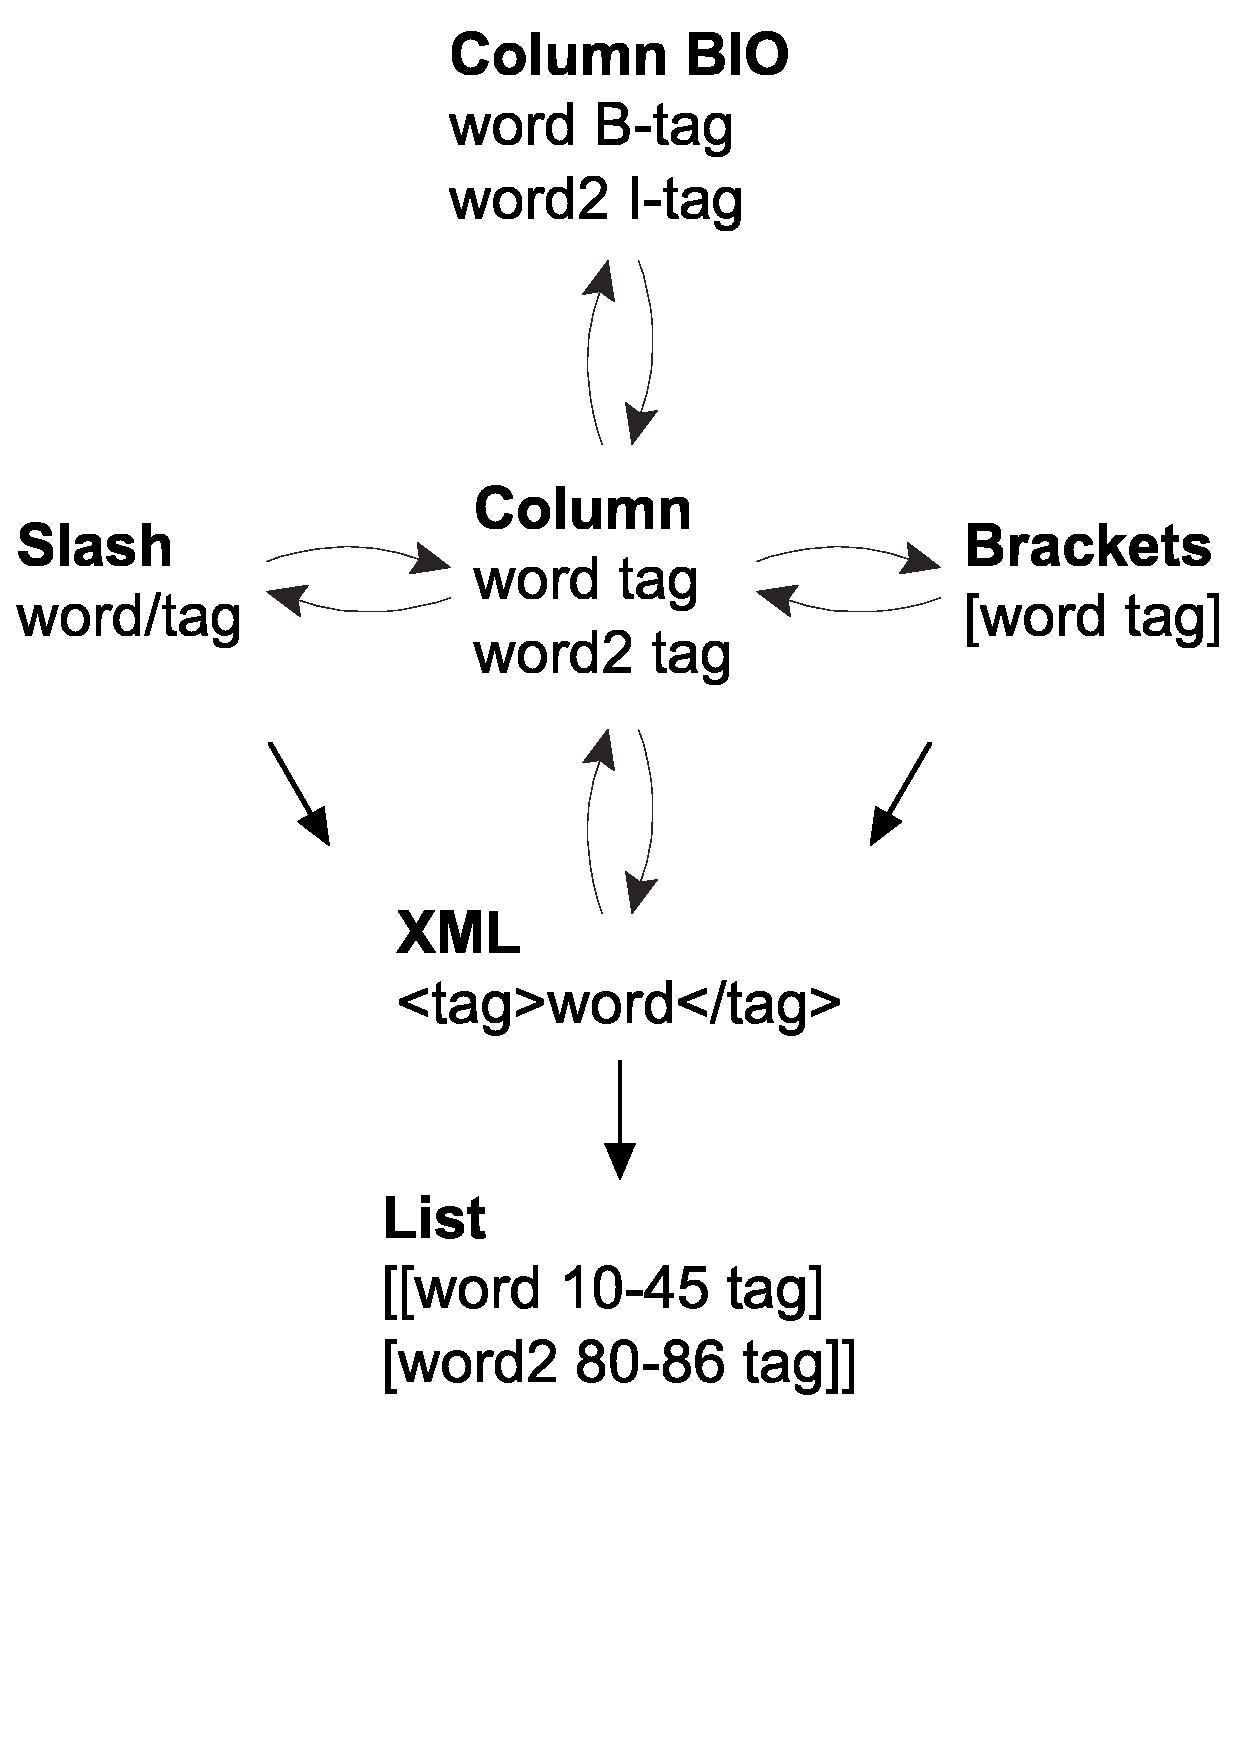
\includegraphics[width=0.5\textwidth]{img/taggingFormats.pdf}
\caption{Possible transformation of tagging formats.}
\label{fig:taggingFormats}
\end{figure}

\paragraph{Using the training set}
Once you have created your training set, you should use the FileFormatParser to transform it into a tab separated column tagging format (if it isn't in this format already).

It is not possible to train a model for the web-based taggers Alchemy and OpenCalais. All other taggers can be trained using the train method, that requires the training file and a model configuration parameter which is different for each tagger.

Let us assume we want to train a model for each trainable tagger to recognize mobile phone names. You should have tagged training data in column separated form as shown below. Usually, the more training data you have, the more stable the trained model. This training data is stored in a tsv file called ``phoneTraining.tsv''.

\begin{verbatim}
The	O
iphone	PHONE
4	PHONE
sells	O
very	O
well O
.	O
\end{verbatim}

Each tagger can be trained as shown in Listing \ref{listing:trainNER}. The only parameter which is used differently for each tagger is the ``modelConfig''. Table \ref{tab:nerConfig} shows what that parameter means for each trainable recognizer.

\begin{table}[ht]
\centering
\begin{tabularx}{\linewidth}{|l|X|X|}
\hline
NER		& Parameter meaning & Example \\
\hline
IllinoisLbjNER	& Path to a configuration file, in this file you can specify which features and parameters should be used and where the trained model should be saved &	.../illinoisner/baselineFeatures.config \\
\hline
JulieNER	& Output path for the trained model. You can add a further parameter with the path to a configuration file, in this file you can specify which features and parameters should be used &	.../juliener/phoneModel.mod and [.../juliener/tutorial/featconfig.conf] \\
\hline
LingPipeNER	& Output path for the trained model &	.../lingpipe/phone.model \\
\hline
OpenNLPNER	& Output path for the trained model, the filename must follow the format ``openNLP\_TAG.bin.gz'' since you can only train one tag per model &	.../opennlp/openNLP\_phone.bin.gz \\
\hline
StanfordNER	& Path to a configuration file, in this file you can specify which features and parameters should be used and where the trained model should be saved &	.../lingpipe/training/austen.prop \\
\hline
TUDNER	& Output path for the trained model &	.../tudner/phoneModel.model \\
\hline
\end{tabularx} 
\caption{Configuration parameters to train named entity recognizers.}
\label{tab:nerConfig}
\end{table}

\begin{codelisting}
\begin{lstlisting}[label=listing:trainNER,caption=Train a named entity recognizer.,frame=tb]
NamedEntityRecognizer ner = new StanfordNER();
boolean successful = ner.train("phoneTraining.tsv", modelConfig);
String output = "successful";
if (!successful) {output = "not successful";}
System.out.println("Training of "+ner.getName()+" was "+output);
\end{lstlisting}
\end{codelisting}

\subsubsection{Evaluating a Tagger}
To see how good a trained tagger performs, we need test data which is tagged in the same manner as the training data. There are different versions of how to evaluate the performance. Let's go through them using an example. For example, let us assume that a human expert created the following markup \cite{nadeau2007yooname}:

\begin{verbatim}
Unlike <PERSON>Robert</PERSON>, <PERSON>John Briggs Jr</PERSON> contacted 
<ORG>Wonderful Stockbrockers Inc</ORG> in <LOCATION>New York</LOCATION> 
and instructed them to sell all his shares in <ORG>Acme</ORG>.
\end{verbatim}

Furthermore, let us assume that a NER system created the following markup \cite{nadeau2007yooname} for the same text:

\begin{verbatim}
<LOCATION>Unlike</LOCATION> Robert, <ORG>John Briggs Jr</ORG> contacted 
Wonderful <ORG>Stockbrockers</ORG> Inc <DATE>in New York</DATE> and 
instructed them to sell all his shares in <ORG>Acme</ORG>.
\end{verbatim}

The only correct match between the correct solution and the NER system output is \verb$<ORG>Acme</ORG>$, all other markups are some kind of errors.

\paragraph{Error Types}
In classification tasks it is often possible to determine the true positives, false positives etc. but in NER it can sometimes help to be more precise about the classes. For example, two false positives are not necessarily equally wrong. Consider a system that had to tag person names in text, and it tagged ``A good start'' and ``Jim Carrey was'' as persons. While the first occurrence is obviously totally wrong, the second has to be considered wrong too but the system only did not find the right hand boundary correctly and tagged the word ``was'' too.
In the previous example we can see five different errors an NER system can make \cite{manning2006nererrors}. The errors are shown and explained in the Table \ref{tab:nererrors} \cite{nadeau2007yooname}.

\begin{table}[ht!]
\centering
\begin{tabularx}{\linewidth}{|X|X|X|}
\hline
Correct Solution	 		& 	System Output	& Error\\
\hline
\hline
Unlike						&	\verb$<LOCATION>Unlike</LOCATION>$	&	The system tagged an entity where there is none.\\
\hline
\verb$<PERSON>Robert</PERSON>$	&	Robert								& 	The system missed to tag an entity.\\
\hline
\verb$<PERSON>John Briggs Jr$ \verb$</PERSON>$	& \verb$<ORG>John Briggs Jr</ORG>$	&	The system tagged the entity but classified it incorrectly.\\
\hline
\verb$<ORG>Wonderful$ \verb$Stockbrockers Inc</ORG>$	&	\verb$<ORG>Stockbrockers</ORG>$	&	The system tagged the entity but the boundaries are wrong.\\
\hline
\verb$<LOCATION>New York$ \verb$</LOCATION>$	&	\verb$<DATE>in New York</DATE>$	&	The system found an entity but classified it incorrectly and got the boundaries wrong.\\
\hline
\end{tabularx} 
\caption{NER features \cite{nadeau2007yooname}.}
\label{tab:nererrors}
\end{table}

Due to the variety of combinations to use the error types, three main evaluation methods have evolved during the years.

\paragraph{Exact-Match Evaluation}
The exact-match evaluation is the most simple one and does not take the different error types into account. A correct assignment must have the boundaries and the classification correct. The final score for the NER system is a micro-averaged f-measure (MAF). The NER system from the example would get the following scores.
\begin{itemize}
\item Precision = Correct / Total Assigned = 1 / 5 = 20\%
\item Recall = Correct / Total Possible = 1 / 5 = 20\%
\item MAF = 20\%
\end{itemize}

\paragraph{MUC Evaluation}
The MUC evaluation method takes all five errors from Table \ref{tab:nererrors} into account and scores a system along two axis, the TYPE and the TEXT axis. If an entity was classified correctly (regardless of the boundaries) the TYPE is assigned correct. If an entity was found with the correct boundaries (regardless of its type) the TEXT is assigned correct. For both axis, three measures are kept: the number of possible entities (POS), the number of actual assigned entities by the system (ACT) and the number of correct answers by the system (COR).
MUC als uses the MAF as the final score for the NER system. As the usual f-measure, also the micro-averaged f-measure is the harmonic mean between precision and recall.
For the example we can calculate the MUC score for the system as follows.
\begin{itemize}
\item COR = 4 (2 times TYPE correct, 2 times TEXT correct)
\item ACT = 10 (5 times TYPE assigned, 5 times TEXT assigned)
\item POS = 10 (5 times TYPE, 5 times TEXT)
\item Precision = COR / ACT = 4 / 10 = 40\%
\item Recall = COR / POS = 4 / 10 = 40\%
\item MAF = 40\%
\end{itemize}

Listing \ref{listing:evaluateNER} shows how we can programmatically evaluate a tagger. 

\begin{codelisting}
\begin{lstlisting}[label=listing:evaluateNER,caption=Evaluating the performance of a named entity tagger.,frame=tb]
// initialize the tagger
NamedEntityRecognizer ner = new TUDNER();

// the path to the test data
String testFilePath = "testData.xml";

// the path to the model that we want to evaluate
String modelPath = "data/models/tudner/phone.model";

// store the evaluation results in an object
EvaluationResult eResult = null;

// evaluate the model using the test data
eResult = ner.evaluate(testFilePath, modelPath, TaggingFormat.XML);

// print out the evaluation result
System.out.println(eResult);

// get interesting values in exact match and MUC mode
String r1 = "F1 Exact: " + eResult.getF1(EvaluationResult.EXACT_MATCH);
String r2 = "F1 MUC: " + eResult.getF1(EvaluationResult.MUC);
System.out.println(r1);
System.out.println(r2);
\end{lstlisting}
\end{codelisting}

\subsection{Web Page Age Detection}
The age of a web page can often be a useful indicator about the freshness of the information. It might also be used in classification or ranking of web documents. Palladian is able to detect the age of many web pages by using four main techniques:
\begin{enumerate}
\item Reading the \textbf{ HTTP header} of a web page and look for the date that the page has changed. Although this information is often absent of incorrect it sometimes is the only date we get.
\item Recognize a date in the \textbf{ URL} of the web page. Especially blogs use the URL style which often reads similar to \texttt{http://domain.tld/posts/YYYY/MM/PostName}. In these cases the date in the domain is a very good indicator of the web page's age.
\item Recognizing and ranking dates in the \textbf{ structure and content} of the web page. Especially news pages start or end their news posts with the location and the date that the event they are reporting about happened. Since many dates might be found in the content it is necessary to rank them among each other. This is done using indicators such as the nearness to certain keywords such as ``published'' for example.
\item Searching for \textbf{ inbound links from archives}. Some web pages can be found in archives with a date. If none of the other techniques returns valuable results it is possible to look up the URL in an archive, although the chances to find it are quite low.
\end{enumerate}

Listing \ref{listing:dateRecognizer} shows how to detect the age of a web page. For more information on the algorithms used, see \cite{gregor2010bachelor}. You can also check out the functionality of the web page age detection online at \url{http://www.webknox.com/wi#detectAge}.

% TODO out of sync with code!
\begin{codelisting}
\begin{lstlisting}[label=listing:dateRecognizer,caption=Detecting the age of a web page.,frame=tb]
// the URL of the page we want to know the age from
String url = "http://www.bbc.co.uk/news/world-europe-11432849";

// ExternalSearch is a boolean to switch on and off reference and
// archive techniques. Standard should be false (off).
boolean externalSearch = false;

// get the highest ranked date for this web page
ExtractedDate date = WebPageDateEvaluator
				.getBestRatedDate(url, externalSearch);

// print the extracted date (should be 29.09.2010)
System.out.println(date);
\end{lstlisting}
\end{codelisting}

%\subsection{FAQ Extractor}
%\textit{ FAQs} are frequently asked questions that are often found on web pages in a structured form. Basically there are three types how the FAQ can be structured:
%\begin{enumerate}
%\item \textbf{ Internal Link} In the beginning of the page, there is a list of questions that each link to the corresponding answer in on the same page.
%\item \textbf{ External Link} In the beginning of the page, there is a list of questions that each link to the the web page that contains the answer.
%\item \textbf{ No Link} Each question is immediately followed by its answer.
%\end{enumerate}
%
%Palladian can handle many FAQs that follow the first or third structure. First, the algorithm detects the XPaths to the questions and then it tries to extract all content between the current and the next question as the answer for the current question.
%
%Listing \ref{listing:faqExtractor} shows how the FAQExtractor can be used programatically. You can also check out the functionality of the FAQ Extractor online at \url{http://www.webknox.com/wi#extractFAQ}.
%
%\begin{codelisting}
%\begin{lstlisting}[label=listing:faqExtractor,caption=Extract an FAQ from a web page.,frame=tb]
%// create a list of question answer pairs
%ArrayList<QA> qas = null;
%
%// the URL that contains the FAQ
%String url = "http://blog.pandora.com/faq/";
%
%// start extracting question and answers from the URL
%qas = QAExtractor.getInstance().extractFAQ(url);
%
%// print the extracted questions and answers
%CollectionHelper.print(qas);
%\end{lstlisting}
%\end{codelisting}

%\subsection{Fact Extraction}
%The FactExtractor can be used to detect facts in tables on web pages given a URL and optionally a small set of seed attribute names that help the extractor. The FactExtractor constructs all XPaths to the seed attributes and compares them. If it recognizes a similarity it concludes that the XPaths that are similar for the seed attributes might also point to other attributes on the page. In case of attributes that are listed in simple tables this approach works pretty well, if the attributes are presented in a more complicated way, the fact extractor might not find anything.
%
%You can also check out the functionality of the FactExtractor online at \url{http://www.webknox.com/wi#extractFacts}.
%
%\begin{codelisting}
%\begin{lstlisting}[label=listing:factExtraction,caption=Extract a list of facts from a web page.,frame=tb]
%// the URL of the facts
%String url = "http://en.wikipedia.org/wiki/Nokia_N95";
%
%// the concept of the attributes
%Concept concept = new Concept("Mobile Phone");
%
%// a small list of seed attributes
%Set<Attribute> seeds = new HashSet<Attribute>();
%int attributeType = Attribute.VALUE_STRING;
%seeds.add(new Attribute("Second camera", attributeType, concept));
%seeds.add(new Attribute("Memory card", attributeType, concept));
%seeds.add(new Attribute("Form factor", attributeType, concept));
%
%// detect the facts using the seeds from the URL
%ArrayList<Fact> detectedFacts = null;
%detectedFacts = FactExtractor.extractFacts(url, seeds);
%		
%// print the extracted facts
%CollectionHelper.print(detectedFacts);
%\end{lstlisting}
%\end{codelisting}

\section{Retrieval}

\subsection{Web Searcher}
The package \texttt{ws.palladian.retrieval.search.web} provides multiple classes that can query a number of search engines with terms and retrieve matching results.

\subsubsection{Basic Features}
The currently supported search engines are:
\begin{itemize}
\item Google, Google Blogs, Google News, Google Images (top 64 results only)\footnote{\url{http://code.google.com/intl/de/apis/websearch/docs/reference.html}}
\item Bing, Bing News, Bing Images (unlimited)\footnote{\url{http://www.bing.com/developers/s/APIBasics.html}}
\item Hakia, Hakia News
\item Tweets on Twitter\footnote{\url{https://dev.twitter.com/docs/api/1/get/search}}
\item Scroogle\footnote{\url{http://www.scroogle.org/}}
\item Blekko\footnote{\url{http://blekko.com}}
\end{itemize}

Some of the search APIs require API keys which can be specified in the \texttt{config/palladian.properties} file or supplied via the constructors of the respective classes. If you need to obtain an API key, check the footnotes from the list above.

\subsubsection{How To}
\label{sec:howto}
The following code snippet shows how to initialize a \texttt{BingSearcher} and a \texttt{GoogleImageSearcher} and get a list of webpages and images for the search query ``Jim Carrey''.
\begin{codelisting}
\begin{lstlisting}[caption=Retrieving results from search engines.,frame=tb]
// create a web searcher for the Bing search engine
WebSearcher<WebResult> searcher = new GoogleSearcher();
// search for "Jim Carrey", 50 results, English language
List<WebResult> webResults = searcher.search("Jim Carrey", 50,
                                       WebSearcherLanguage.ENGLISH);
// print the results
CollectionHelper.print(webResults);
    
// create a web searcher to search for images on Google
WebSearcher<WebImageResult> imageSearcher = new GoogleImageSearcher();
// search for ten images with "Jim Carrey"
List<WebImageResult> imageResults = imageSearcher.search("Jim Carrey", 10);
// print the results
CollectionHelper.print(imageResults);
\end{lstlisting}
\end{codelisting}

\subsection{Document Retriever}
The \emph{DocumentRetriever} can be used do download documents from the WWW or create W3C documents from (X)HTML files from the hard disk. 

\subsubsection{Basic Features}
Basic functionalities include:
\begin{itemize}
\item Download and save contents of a web page.
\item Download documents in parallel using threads.
\item Use \verb#DownloadFilter# to specify which contents are allowed.
\item Switch proxies after a certain number of requests to avoid being blocked
\end{itemize}

\subsubsection{How To}
The following code shows how to instantiate a simple \verb#DocumentRetriever#.

\begin{codelisting}
\begin{lstlisting}[caption=Using the web crawler.,frame=tb]
// create the object
DocumentRetriever retriever = new DocumentRetriever();
   
// download and save a web page including their headers in a gzipped file
retriever.downloadAndSave("http://cinefreaks.com", "page.gz", true);
   
// create a retriever that is triggered for every retrieved page
RetrieverCallback crawlerCallback = new RetrieverCallback() {
     @Override
     public void onFinishRetrieval(Document document) {
          // do something with the page
          LOGGER.info(document.getDocumentURI());
     }
};
retriever.addRetrieverCallback(crawlerCallback);
   
// set the maximum number of threads to 10
retriever.setMaxThreads(10);
   
// the retriever should automatically use different proxies
// after every 3rd request (default is no proxy switching)
retriever.setSwitchProxyRequests(3);
   
 // set a list of proxies to choose from
List<String> proxyList = new ArrayList<String>();
proxyList.add("83.244.106.73:8080");
proxyList.add("83.244.106.73:80");
proxyList.add("67.159.31.22:8080");
retriever.setProxyList(proxyList);
        
// give the retriever a list of URLs to download
retriever.add("http://www.cinefreaks.com");
retriever.add("http://www.imdb.com");
        
// download documents
Set<Document> documents = retriever.start();
CollectionHelper.print(documents);
     
// or just get one document
Document webPage = retriever.getWebDocument("http://www.cinefreaks.com");
LOGGER.info(webPage.getDocumentURI());
\end{lstlisting}
\end{codelisting}

\subsection{Web Crawler}
The web crawler can be used to crawl domains or the web in general.

\subsubsection{Basic Features}
Basic functionalities include:
\begin{itemize}
\item Automatically crawl in- and/or outbound links from web pages.
\item Use URL rules for the crawling process.
\end{itemize}

\subsubsection{How To}
The following code shows how to instantiate a simple crawler that starts at http://www.dmoz.org and follows all in- and outbound links. The URL of each crawled page is printed to the screen. The crawler will use 10 threads, changes the proxy after every third request and stops after having crawled 1000 pages. Instead of setting the parameters using the code, we can also specify them in the config/palladian.properties file.

\begin{codelisting}
\begin{lstlisting}[caption=Using the web crawler.,frame=tb]
// create the crawler object
Crawler crawler = new Crawler();

// create a callback that is triggered for every crawled page
RetrieverCallback crawlerCallback = new RetrieverCallback() {
    @Override
    public void onFinishRetrieval(Document document) {
        LOGGER.info("downloaded the page " + document.getDocumentURI());
    }
};
crawler.addCrawlerCallback(crawlerCallback);

// stop after 1000 pages have been crawled (default is unlimited)
crawler.setStopCount(1000);

// set the maximum number of threads to 1
crawler.setMaxThreads(1);

// the crawler should automatically use different proxies after every
// 3rd request (default is no proxy switching)
crawler.getDocumentRetriever().setSwitchProxyRequests(3);

// set a list of proxies to choose from
List<String> proxyList = new ArrayList<String>();
proxyList.add("83.244.106.73:8080");
proxyList.add("83.244.106.73:80");
proxyList.add("67.159.31.22:8080");
crawler.getDocumentRetriever().setProxyList(proxyList);

// start the crawling process from a certain page, true = follow links
// within the start domain, true = follow outgoing links
crawler.startCrawl("http://www.dmoz.org/", true, true);
\end{lstlisting}
\end{codelisting}

\subsection{Web Feeds}
Palladian's \texttt{ws.palladian.web.feeds} package offers various functionalities for tasks related to RSS and Atom web feeds. The most important classes include:

\begin{itemize}

	\item \texttt{FeedDownloader} can be used for retrieving web feeds. The class basically wraps ROME library~\cite{rome} for feed parsing but adds some additional techniques and fallbacks for parsing non-standard and malformed feeds, which ROME normally cannot parse.

	\item \texttt{FeedReader} is responsible for continuously aggregating web feeds using various different algorithms to predict feed's update behaviours.

	\item \texttt{FeedDiscovery} allows searching for web feeds using standard web search engines like Yahoo! and the so called ``autodiscovery'' feature\footnote{\url{http://diveintomark.org/archives/2003/12/19/atom-autodiscovery} (also works for RSS)}, to detect feeds on web pages.

	\item \texttt{FeedDatabase} implements the feed's package persistence layer using a relational database. The necessary MySQL database schema can be found in \texttt{config/feedsDbSchema.sql}\footnote{You can use phphMyAdmin or MySQL command line utilities to import the schema into your database.}.

	\item \texttt{FeedImporter} is used for adding new web feeds to the database.

	\item The class \texttt{Feed} and its associated \texttt{FeedItem}s model a web feed's data structure.

\end{itemize}

Code Listing~\ref{listing:feeds} gives a minimal sample use case employing the described classes.

\begin{codelisting}
\begin{lstlisting}[caption=Using the \texttt{feeds} package.,frame=tb,label=listing:feeds]
// search feeds for "Porsche 911"
String discoveredFeedsFile = "data/foundFeeds.txt";
FeedDiscovery feedDiscovery = new FeedDiscovery();
feedDiscovery.setSearchEngine(new BingSearcher());
feedDiscovery.setResultFilePath(discoveredFeedsFile);
feedDiscovery.addQuery("Porsche 911");
feedDiscovery.setNumResults(100);
feedDiscovery.findFeeds();

// download a feed
FeedParser feedParser = new RomeFeedParser();
Feed feed = feedParser.getFeed("http://rss.cnn.com/rss/edition.rss");
List<FeedItem> feedItems = feed.getItems();
CollectionHelper.print(feedItems);

// initialize the FeedDatabase for storing the data
FeedStore feedStore = DatabaseManagerFactory.create(FeedDatabase.class);

// add some feed URLs to the database
FeedImporter feedImporter = new FeedImporter(feedStore);
feedImporter.addFeedsFromFile(discoveredFeedsFile);

// start aggregating news for the feeds in the database
FeedReader feedReader = new FeedReader(feedStore);
feedReader.aggregate();
\end{lstlisting}
\end{codelisting}

\subsection{Wiktionary Database}\label{sec:wiktionaryDB}
Palladian offers a simple interface to the Wiktionary\footnote{\url{http://www.wiktionary.org/}} data. So far, there are two databases available, one in German and one in English. The database contains information about each word. This information is in particular:
\begin{itemize}
\item Language, the language of the word. For example, English, German, Spanish...
\item Type, the type of the word. For example, Noun, Adjective, Verb...
\item Synonyms, words which have a similar meaning. For example, notebook = laptop.
\item Hypernyms, words which are ancestrally related to the word. For example, notebook => computer. Hypernyms are only in the German DB since the English Wiktionary does not provide them.
\end{itemize}

Code Listing~\ref{listing:wiktionary} shows how to access the database. We create the WordDB with the path to the stored database. Then we can query the database with a string and in case the word is found we get a Word object holding basic information such as language and type. We can then call \verb+aggregateInforamtion(word)+ to find synonyms and hypernyms belonging to the word.

\begin{codelisting}
\begin{lstlisting}[caption=Using the interface to the Wiktionary WordDB.,frame=tb,label=listing:wiktionary]
// load a word DB
WordDB wordDB = new WordDB("data/models/wordDatabaseEnglish/");

// you can load the database into the memory for faster read access
// wordDB.loadDbToMemory();

// search a word in the dtabase
Word word = wordDB.getWord("freedom");
LOGGER.info(word);

// find synonmys and hypernyms for the word
wordDB.aggregateInformation(word);
LOGGER.info(word);
\end{lstlisting}
\end{codelisting}

Other languages from the Wiktionary project can be parsed after extending the WiktionaryParser. The Wiktionary dumps can be found at \url{http://dumps.wikimedia.org/backup-index.html}.

\subsection{MediaWiki Crawler}\label{sec:MWCrawler}
The MediaWiki crawler can be used to retrieve content and metadata from Wiki pages. This component is not really a crawler since it uses the MediaWiki API \cite{MWAPI2011} to get all information, anyhow, we call it a crawler. To communicate with the API, the crawler is based on the Java Wiki Bot Framework (jwbf) \cite{jwbf2011}. 

\subsubsection{Basic Features}
Basic functionalities include:
\begin{itemize}
\item Download the content of a complete wiki.
\item Store content in relational data base.
\item Select namespaces to crawl.
\item Access login protected Wikis.
\item For a single page, extract: 
	\begin{itemize}
	\item page title,
	\item HTML content of the most recent version, rendered by wiki (without navigation bar on left side),
	\item complete history, for every revision: revisionID, timestamp of modification and author,
	\item all links to other pages within the same wiki.
	\end{itemize}	
\item Contineous crawling, i.e. keep data base up to date.
\item Crawl multiple Wikis in parallel.
\item Notification to process new pages in your own code.
\end{itemize}

\subsubsection{Architecture}

Figure~\ref{fig:MWCrawler-architecture} shows the architecture of the MediaWiki crawler. The classes \emph{MediaWikiCrawler} and \emph{PageConsumer} are the central classes, holding the control flow for fetching pages from the wiki (MediaWikiCrawlerfrom) and processing the extracted data (PageConsumer), for details see~\ref{sec:mw_extend}. Package \emph{data} provides classes to temporary store fetched pages and their metadata while package \emph{persistence} is used as a persistance layer to store extracted data in a database and load the crawler configuration. Package \emph{queries} extends some queries of the Java Wiki Bot Framework (jwbf). All communication with the MediaWiki API is done via jwbf. 

\begin{figure}[ht!]
\centering
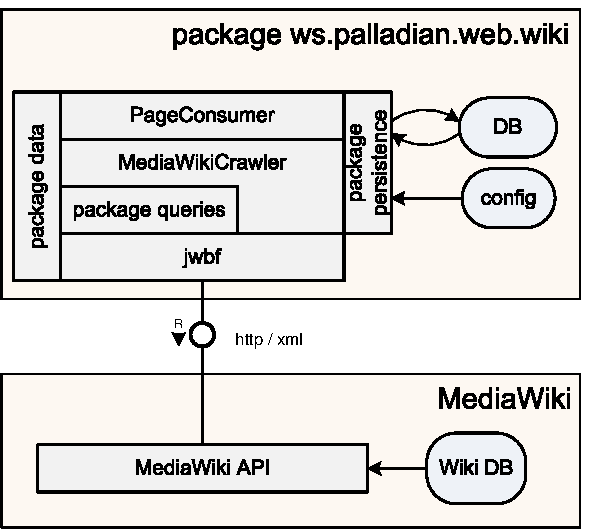
\includegraphics[width=0.6\textwidth]{img/MediaWiki_Crawler_Architecture.pdf}
\caption{MediaWiki crawler architecture.}
\label{fig:MWCrawler-architecture}
\end{figure}

\subsubsection{How To}
The necessary MySQL database schema can be found in \texttt{config/mwCrawlerDbSchema.sql}, the crawler's configuration can be found in \texttt{config/mwCrawlerConfiguration.yml}, see \ref{listing:MWCrawler_config}. For every Wiki to crawl, at least \emph{wikiName} and \emph{wikiURL} are required.

\begin{codelisting}
\begin{lstlisting}[caption=MediaWiki crawler configuration.,frame=tb,language=tex,breaklines=true,label=listing:MWCrawler_config]
# sample
    # Unique name of this wiki, like "Wikipedia (en)". Required parameter.
- wikiName: "Wikipedia (en)"
    # Path to the Wiki, like "http://en.wikipedia.org/". Required parameter.
  wikiURL: "http://en.wikipedia.org/"
    # Path to api.php, relative from wikiURL, like "/w/" for wikipedia. Must not contain the file name api.php.
    # Do not forget the "/" in  the end of the path if there is any.
    # Optional parameter. Leave empty if unknown. 		
  pathToAPI: "/w/" 
    # Path to wiki pages, relative from wiki_url, like /wiki/ as used in wikipedia (resulting path is http://de.wikipedia.org/wiki/).         
    # Do not forget the "/" in  the end of the path if there is any. 
    # Optional parameter. Leave empty if unknown.
  pathToContent: "/wiki/"
    # User name to use for crawling.
    # Optional parameter. 
  crawlerUserName: "myname" 
    # The user's password. Optional parameter. 
  crawlerPassword: "mysecret"
    # The namespaceIDs to include into crawling, separated by comma ",". All pages within these namespaces are crawled.
    # namespaceIDs that do not exist in the Wiki are ignored.
    # known bug: to crawl a single namespace, add comma like "1,", otherwise all namespaces are crawled! 
    # Optional parameter. Leave empty to crawl all namespaces.
  namespacesToCrawl: "0, 1, 12" 
\end{lstlisting}
\end{codelisting}

To run the MediaWiki crawler, do the following three steps: 
\begin{enumerate}
	\item Create the required database tables by executing mwCrawlerDbSchema.sql.
	\item Change the configuration mwCrawlerConfiguration.yml to setup all Wikis to crawl.
	\item Start the crawler like in listing~\ref{listing:MWCrawler_initialize}.
\end{enumerate}  

\begin{codelisting}
\begin{lstlisting}[caption=MediaWiki crawler initialization.,frame=tb,breaklines=true,label=listing:MWCrawler_initialize]
final int queueCapacity = 1000;
final int pageConsumers = 5;

LinkedBlockingQueue<WikiPage> pageQueue = new LinkedBlockingQueue<WikiPage>(queueCapacity);
MWConfigLoader.initialize(pageQueue);
for (int i = 1; i <= pageConsumers; i++) {
  Thread consumer = new Thread(new PageConsumer(pageQueue), "Consum-" + i);
  consumer.start();
}
\end{lstlisting}
\end{codelisting}

\subsubsection{Understand and extend the crawler}\label{sec:mw_extend}

As already introduced, the crawler has two central classes---MediaWikiCrawler and PageConsumer---to control the work flow. For every wiki to crawl one MediaWikiCrawler is created, running as a thread, "producing" \emph{WikiPage}-objects when fetching a new page or revision and adding them to a central \emph{pageQueue}. PageConsumer-threads wait for new pages and are used to process the extracted data. The current PageConsumer implementation contains basic functionality only, it has to be extended (inheritance). Override \emph{consume(WikiPage page)} to do something useful with every page that is taken from the pageQueue. 

The MediaWikiCrawler itself should not be changed unless more information (e.g. the page content of every revision) is required. Figure~\ref{fig:MWCrawler-state_machine} shows the state machine of the crawler. The initialization is done by \emph{MWConfigLoader} which loads the configuration from data/mwCrawlerConfiguration.yml, updates the configuration in the database and starts one MediaWikiCrawler-thread per Wiki to crawl. Every MediaWikiCrawler does the following: 

\textbf{first start}: If the crawler is started the first time, it gets all namespaces from the API and stores them in the database. Depending on the parameter \emph{namespacesToCrawl} in mwCrawlerConfiguration.yml, all or the selected namespaces are marked for crawling. The next step is to fetch the titles of all page from the API. Next, for each title, the page content, Wiki-links to other pages in the same Wiki and all revisions are fetched from the API. As soon as a page has been processed completely, it is put to the pageQueue to be processed by one of the PageConsumers. When done, the crawler writes the current time to database and enters a continuous crawling mode. Caution: On startup, every crawler checks whether this Wiki has been crawled completely before. If not, it deletes all page-reated data from database. 

\textbf{wiki already crawled}: If the wiki has already been crawled completely, the crawler enters the continuous crawling mode. It wakes up periodically and checks the Wiki for new pages and new revisions of existing pages. Every new/updated page is added to the pageQueue.

\begin{figure}[htb]
\centering
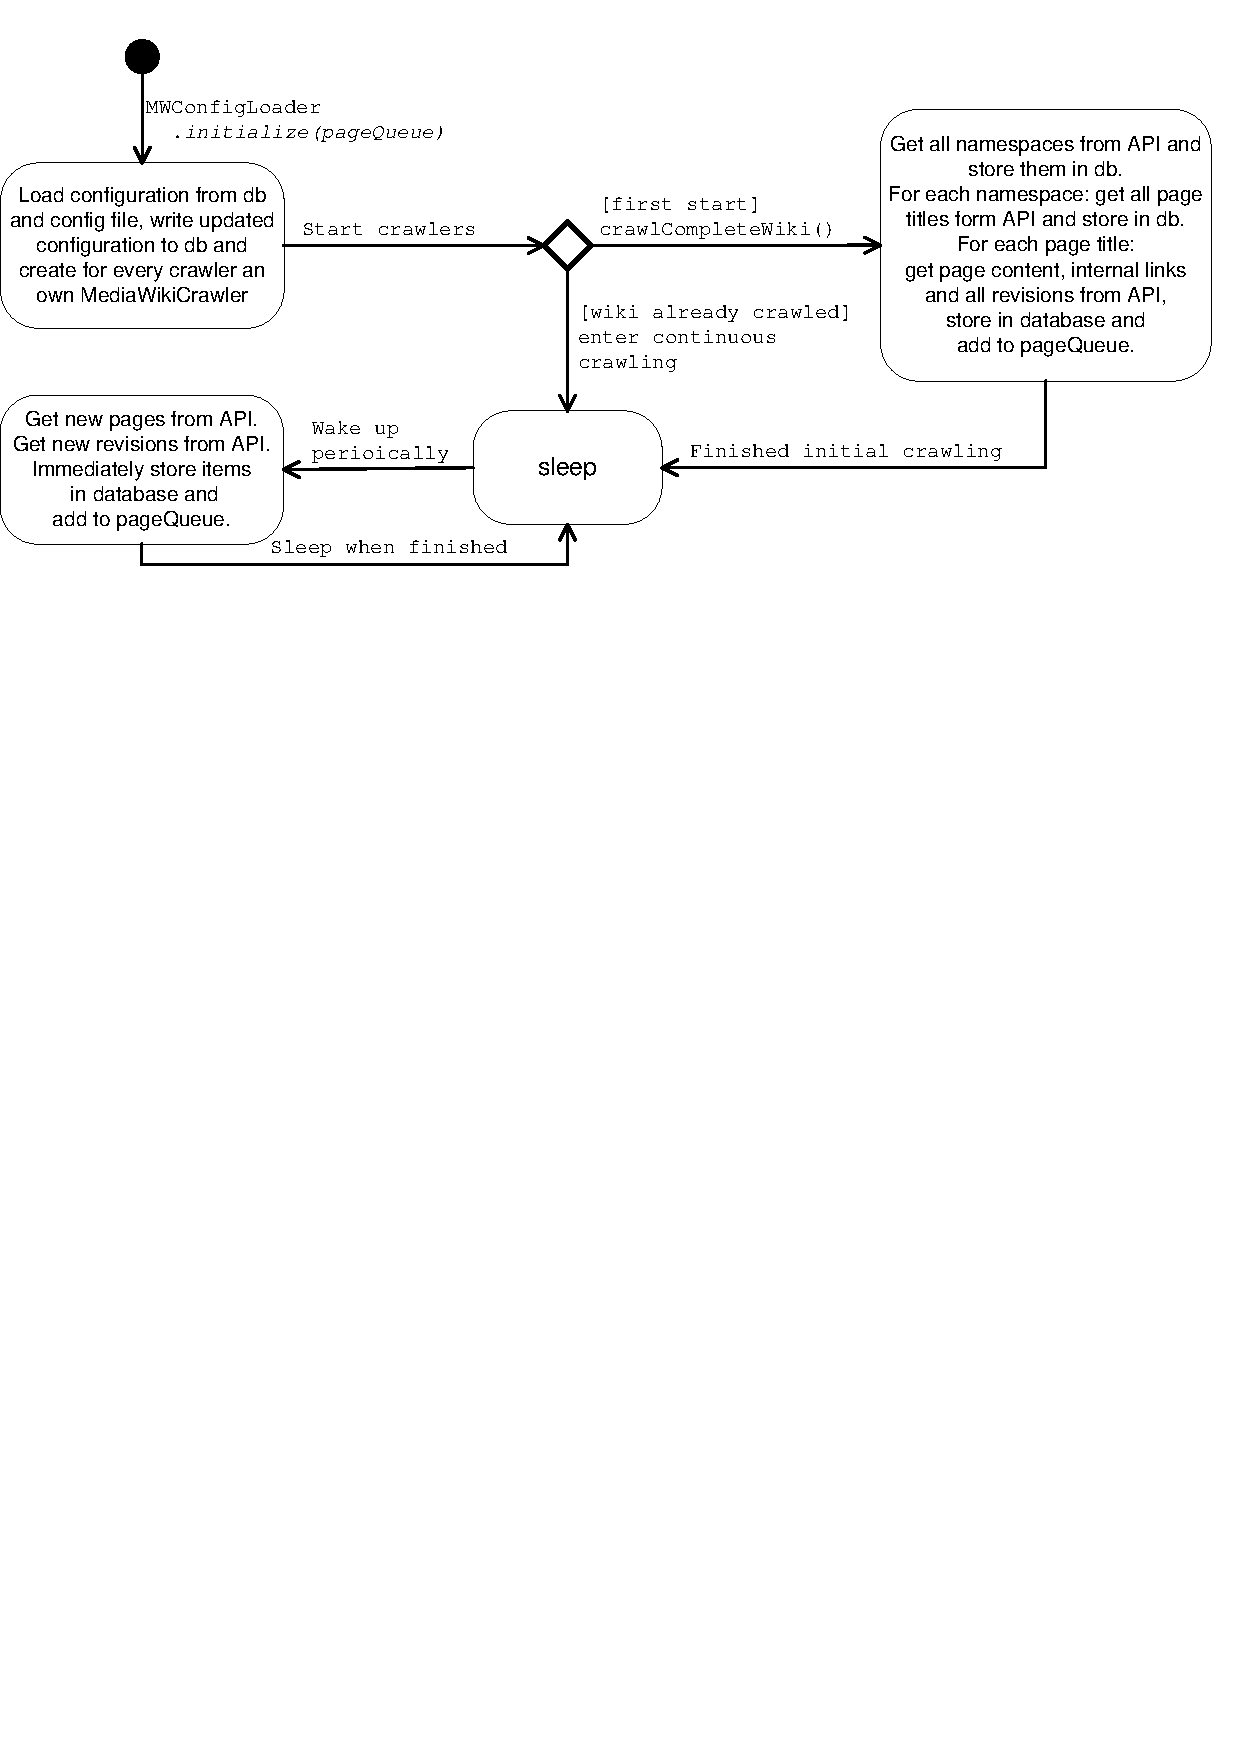
\includegraphics[width=\textwidth]{img/MediaWikiCrawler-UMLStateMachine.pdf}
\caption{MediaWiki crawler UML state machine.}
\label{fig:MWCrawler-state_machine}
\end{figure}

% bis hier 67 S�tze

\section{Preprocessing}
\subsection{Tokenization}
A \textit{Token} is a sequence of characters that can be categorized according to the tokenization rules. \textit{Tokenization} is the process of transforming a text into a sequence of tokens. Table \ref{tab:tokenTypes} shows example token types. The text ``Today I lost \$1000 dollar playing poker.'' could consists of 8 tokens for example. What token types exist depend on the application. The dollar sign could be a single token for example. Palladian uses regular expressions to perform the tokenization.

\begin{table}[ht!]
\centering
\begin{tabular}{|l|l|}
\hline
Character sequence		& Token type \\
\hline
many			& word \\
\hline
\$1000		& amount of money  \\
\hline
26.09.2010	& date \\
\hline
.				& punctuation \\
\hline
\end{tabular} 
\caption{Example types of tokens.}
\label{tab:tokenTypes}
\end{table}

One can also see each sentence of a text as a token, in this case the tokenization process is called sentence splitting as explained int he next section.

\subsection{Sentence Splitting}
Palladian has a rudimentary implementation for the common need for sentence splitting. Palladian implementation works with hand-crafted rules and thus does not require a model. Sentences try to be splitted on periods, question marks, and exclamation marks but there are also rules that try to prevent splitting sentences at ellipses. For example, the following is online one sentence although it contains several periods: ``Sometimes sentenes contain many periods...really!''.

The following code shows how the sentence splitting can be used:
\begin{codelisting}
\begin{lstlisting}[caption=Using the sentence splitter.,frame=tb]
String inputText = "This is a sentence. This is another one!";
List<String> sentences = Tokenizer.getSentences(inputText);
CollectionHelper.print(sentences);
// prints:
// This is a sentence
// This is another one!
\end{lstlisting}
\end{codelisting}

You can also get a specific sentence by providing a phrase that is part of the sentence using the $getSentence$ method.

\subsection{Creating N-Grams}
\label{sec:ngrams}

N-grams are sets of tokens of the length n. We can distinguish two main types of n-grams:

\begin{enumerate}
\item \textbf{Character level n-grams} use each character of the string as a token. For example, from the string ``It is sunny'' we can create the following set of 3-grams: ${it ,t i, is,is ,s s, su,sun,unn,nny}$. The number of n-grams in a set can be calculated as $ngrams = numberOfTokens - n + 1$. In our example that means $9 = 11 - 3 + 1$.
\item \textbf{Word level n-grams} use each word (separated with white space) of the string as a token. For example, from the string ``It is so nice and sunny today'' we can create the following set of 3-grams: ${It is so,is so nice,so nice and,nice and sunny,and sunny today}$. The number of n-grams in a set can be calculated as $ngrams = numberOfTokens - n + 1$. In our example that means $5 = 7 - 3 + 1$. If you want to have single words as features for the text classifier you can simply use unigrams or bigrams which are n-grams with $n=1$ or $n=2$ respectively.
\end{enumerate}

The document preprocessor allows you to create a set of n-grams with different length too. For example, you can create all 2-grams, 3-grams, and 4-grams for the given input text.

Listing \ref{listing:ngrams} shows how you can create n-grams from a given text.

\begin{codelisting}
\begin{lstlisting}[label=listing:ngrams,caption=Creating n-grams.,frame=tb]
// the input text that we want to separate into n-grams
String inputText = "a cat runs funnily";

// store a set of n-grams
Set<String> ngrams = null;

// calculate all character n-grams of length 3
ngrams = Tokenizer.calculateCharNGrams(inputText,3);

// calculate all word n-grams of length 3
ngrams = Tokenizer.calculateWordNGrams(inputText,3);

// calculate all character level n-grams of length 3 to 5
ngrams = Tokenizer.calculateAllCharNGrams(inputText,3,5);

// calculate all character word n-grams of length 1 to 3
ngrams = Tokenizer.calculateAllWordNGrams(inputText,1,3);
\end{lstlisting}
\end{codelisting}

\subsection{Noun Pluralization and Singularization}
Palladian is able to transform most English singular nouns to their plural and back. For example, ``city'' becomes ``cities'' and ``index'' becomes ``indices''.

Listing \ref{listing:singularPlural} shows the simple usage of the singularization and pluralization using the WordTransformer class.

\begin{codelisting}
\begin{lstlisting}[label=listing:singularPlural,caption=Transforming words from singular to plural and vice versa.,frame=tb]
String singular = "city";
String plural = "";
plural = WordTransformer.wordToPlural(singular);
singular = WordTransformer.wordToSingular(plural);
System.out.println(singular);
System.out.println(plural);
// prints:
// cities
// city
\end{lstlisting}
\end{codelisting}

\section{Miscellaneous}
The toolkit contains many helper functionalities for reoccurring tasks in the \texttt{ws.palladian.helper} package. The following code snippet shows several sample usages of some of the functions.

\begin{codelisting}
\begin{lstlisting}[caption=Miscellaneous functions.,frame=tb]
// sort a map by its value in ascending order (2nd parameter = true)
Map m = CollectionHelper.sortByValue(map, true);

// reverse a list
List l = CollectionHelper.reverse(list);

// print the contents of a collection
CollectionHelper.print(collection);

// get the runtime of an algorithm and print it (2nd parameter = true)
long startTime = System.currentTimeMillis();
for (int i = 0; i < 10000; i++) {
	int c = i * 2;
}
DateHelper.getRuntime(t1, true);

// (de) serialization of objects
FileHelper.serialize(obj, "obj.ser");
Object obj = FileHelper.deserialize("obj.ser");

// rename, copy, move and delete files
FileHelper.rename(new File("a.txt"), "b.txt");
FileHelper.copyFile("src.txt", "dest.txt");
FileHelper.move(new File("src.txt"), "dest.txt");
FileHelper.delete("src.txt");

// get files from a folder
File[] files = FileHelper.getFiles("folder");

// zip and unzip a text
FileHelper.zip("text", "zipFile.zip");
String t = FileHelper.unzipFileToString("zipFile.zip");

// perform some action on every line of an ASCII file
final Object[] obj = new Object[1];
obj[0] = 1;

LineAction la = new LineAction(obj) {
  
    @Override
    public void performAction(String line, int lineNumber) {
        System.out.println(lineNumber + ": " + line + " " + obj[0]); 
    }
}
FileHelper.performActionOnEveryLine(filePath, la);

// round a number with a number of digits
double r = MathHelper.round(2.3333, 2);

// remove HTML tags
String r = HTMLHelper.removeHTMLTags("<a>abc</a>",
                                       true, true
                                       true, true);

// trim a string
String t = StringHelper.trim(" _to trim++++");

// reverse a string
String r = StringHelper.reverse("abc");

// encode and decode base64
String e = StringHelper.encodeBase64("abc");
String d = StringHelper.decodeBase64(e);

\end{lstlisting}
\end{codelisting}

\section{Persistence}

Working with JDBC can be annoying and error prone as one has to deal with SQLExceptions and take care of closing open resources to avoid memory leaks which leads to loads of boilerplate code. Of course, we are not the first to stumble over these issues; the Java Persistence API (JPA) and frameworks like Hibernate or 	EclipseLink provide sophisticated solutions for dealing with relational databases. Nevertheless we have made the experience, that the power offered by these frameworks comes with a big portion of black magic, making it hard to understand how they work internally, which can lead to plenty of frustration.

Because of that, we provide our own light weight ORM implementation with Palladian which can be found in \texttt{ws.palladian.persistence}. The class \texttt{DatabaseManager} offers various methods for working with SQL databases. For specific applications, it is intended to subclass \texttt{DatabaseManager} and to add domain specific persistence operations. Instances of \texttt{DatabaseManager} and its subclasses are created using the \texttt{DatabaseManagerFactory}, which takes care of proper configuration and provides database connections using the BoneCP\footnote{\url{http://jolbox.com/}} connection pool library.

Processing and transforming database results can be simplified by subclassing or implementing \texttt{ResultCallback}s and \texttt{RowConverter}s. While the first provides a simple callback for results from database rows, the latter goes a step further and transforms database rows to arbitrary domain objects. \texttt{ResultIterator}s can be used for iterating over big amounts of database results.

For a minimal example on the usage of the persistence mechanism, see the following listings. Listing~\ref{lst:persistence1} shows a typical domain class which we want to persist. Listing~\ref{lst:persistence2} is a domain specific \texttt{DatabaseManager} subclass. The conversion from the database rows to the domain objects is done by the \texttt{RowConverter} implementation given in Listing~\ref{lst:persistence3}. Listing~\ref{lst:persistence4} gives a short example on how to use the persistence mechanism.

\begin{codelisting}
\begin{lstlisting}[label=lst:persistence1,caption=Domain class]
class Cat {
    private String name;
    private String color;

    public Cat(String name, String color) {
        this.name = name;
        this.color = color;
    }

    @Override
    public String toString() {
        return "Cat [name=" + name + ", color=" + color + "]";
    }
}
\end{lstlisting}
\end{codelisting}

\begin{codelisting}
\begin{lstlisting}[label=lst:persistence2,caption=Domain specific database manager]
class CatDatabase extends DatabaseManager {

    private static final String ADD_CAT = 
               "INSERT INTO cats SET name = ?, color = ?";
    private static final String GET_CATS = "SELECT * FROM cats";
    private static final String GET_CAT_BY_NAME = 
               "SELECT * FROM cats WHERE name = ?";

    protected CatDatabase(ConnectionManager connectionManager) {
        super(connectionManager);
    }

    public boolean saveCat(Cat cat) {
        return runInsertReturnId(
               ADD_CAT, cat.getName(), cat.getColor()) > 0;
    }

    public List<Cat> getCats() {
        return runQuery(new CatRowConverter(), GET_CATS);
    }

    public Cat getCat(String name) {
        return runSingleQuery(
               new CatRowConverter(), GET_CAT_BY_NAME, name);
    }
}
\end{lstlisting}
\end{codelisting}
	
\begin{codelisting}
\begin{lstlisting}[label=lst:persistence3,caption=Row converter for domain objects]
class CatRowConverter implements RowConverter<Cat> {
    @Override
    public Cat convert(ResultSet resultSet) throws SQLException {
        String name = resultSet.getString("name");
        String color = resultSet.getString("color");
        return new Cat(name, color);
    }
}
\end{lstlisting}
\end{codelisting}

\begin{codelisting}
\begin{lstlisting}[label=lst:persistence4,caption=Usage example]
CatDatabase catDatabase = 
       DatabaseManagerFactory.create(CatDatabase.class, getConfig());

catDatabase.saveCat(new Cat("Snowball 1", "black"));
catDatabase.saveCat(new Cat("Snowball 2", "grey"));
catDatabase.saveCat(new Cat("Snowball 3", "dark grey"));

CollectionHelper.print(catDatabase.getCats());

System.out.println(catDatabase.getCat("Snowball 1"));
\end{lstlisting}
\end{codelisting}
